\section*{\FIRSTkit capabilities}

The widespread adoption of \R as a tool for statistical analysis has undoubtedly been an important development for the scientific community. However, using \R in most cases still requires a basic knowledge of programming concepts which may pose a steep learning curve for the introductory statistics student (Tan, Ting, and Ling 2009). The website is organized around the idea in how introductory statistics courses are carry. \FIRSTkit capabilities are descriptive statistics, inference and regression. In terms of the descriptive statistics, the user can obtain location summaries as well dispersion. 

\subsection{Descriptive Statistics}

Describing (or summarizing) a data in a clear in a concise way is one of the first things we usually taught in a introductory statistics courses. Many methods are available for summarizing data in both numeric and graphical form. \FIRSTkit allow to obtain summary regarding location and dispersion. In terms of location these are sample mean, trimmed mean, median, and geometric mean. Given a sample of size $n$, consider independent random variables $X_1, X_2,\ldots, X_n$ that we wish to summarized. 

\subsubsection{Location Measurements}

\begin{figure}
  \centering
  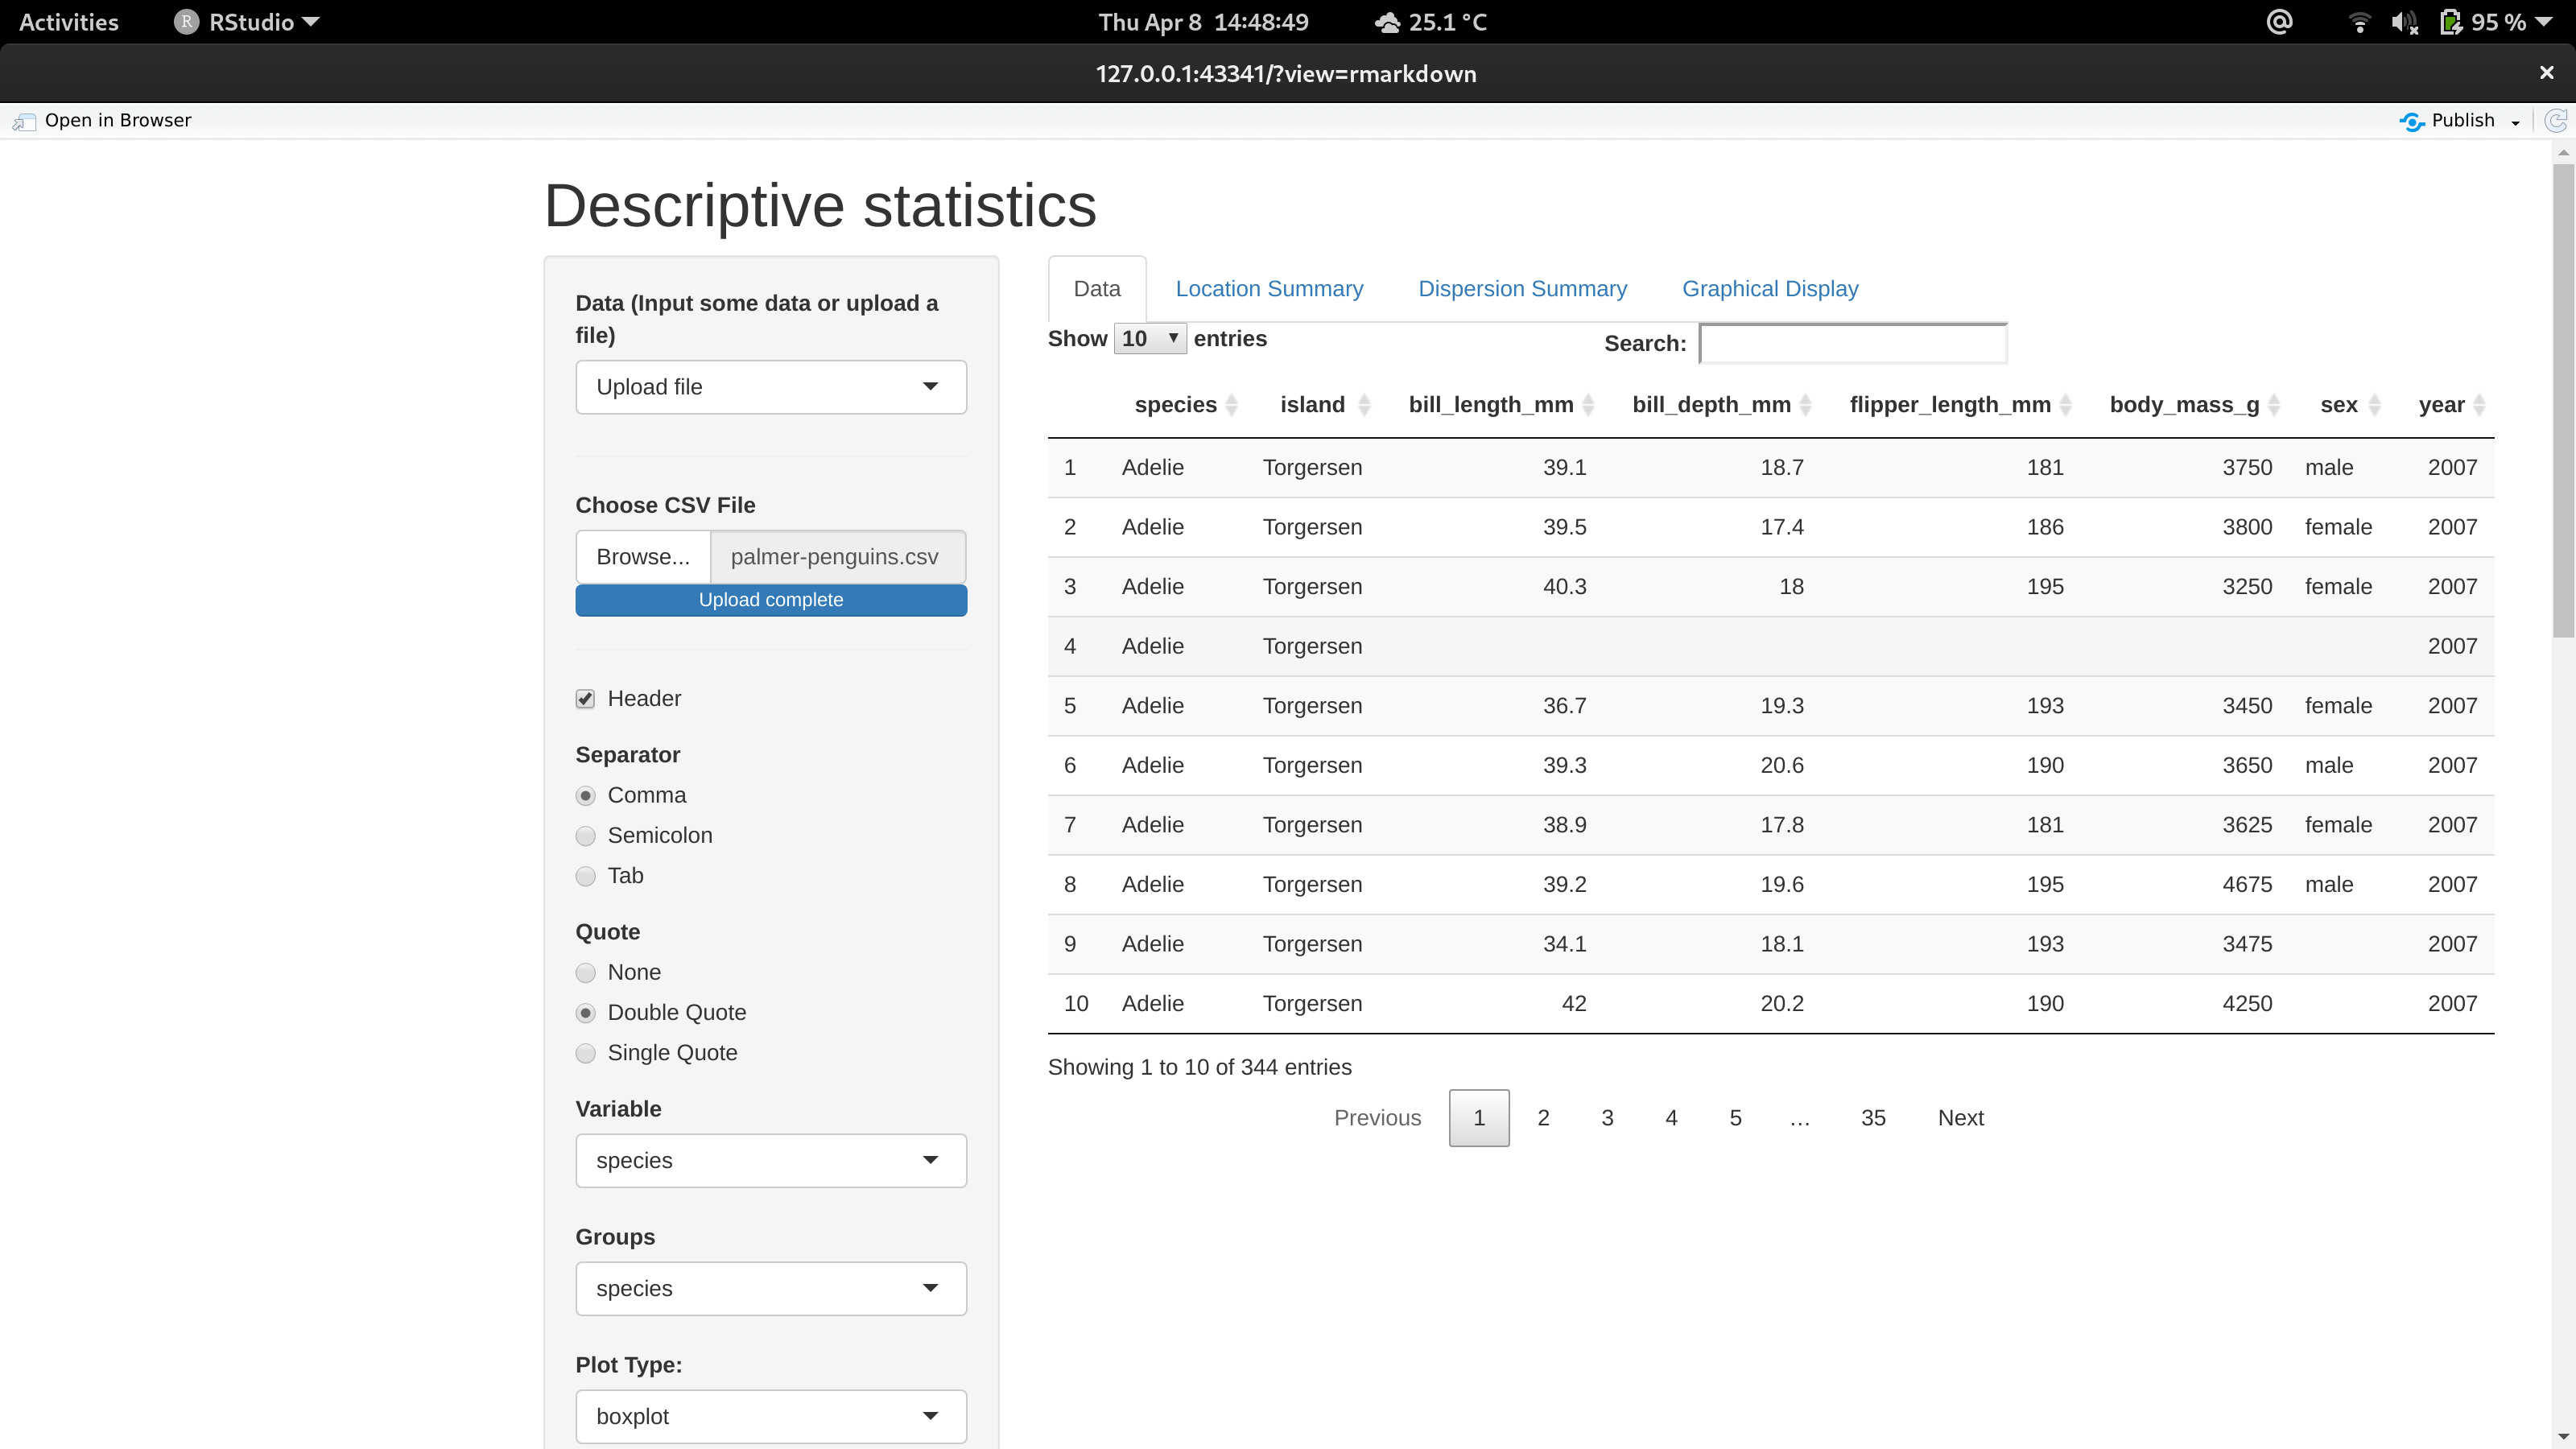
\includegraphics[width=\textwidth]{figures/Descriptive1}
  \end{figure}
\begin{enumerate}
\item {\bf Arithmetic mean}: The sample mean from a group of observations is an estimate of the population mean $\mu$.  The sample mean is defined to be,
\[
\bar{x}= \frac{1}{n}\sum^n_{i=1}x_i
\]
\item Trimmed mean: This mean is computed after discarding given parts of a probability distribution or sample at the high and low end, and typically discarding an equal amount of both. This number of points to be discarded is usually given as a percentage of the total number of points, but may also be given as a fixed number of points. 
\begin{enumerate}
\item First find $n =$ number of observations.
\item Reorder them as ``order statistic''' $X_i$ from the smallest to the largest.
\item Find lower case $p=P/100$ = proportion trimmed.
\item Compute $np$. If $np$ is an integer use $k=np$ and trim $k$ observations at both ends. $R = \mbox{remaining observations} = n-2k$. The trimmed mean is defined as,
\[
\bar{x}_{k} = \frac{X_{k+1}+X_{k+2}+\cdots+X_{n-k}}{R} 
\]
\end{enumerate}
\item Median: Middle value separating the greater and lesser halves of a data set ,
\[
M = X_{(0.5 \times n)}
\]
\item Geometric Mean: The geometric mean of a non-empty data set of (positive) numbers is always at most their arithmetic mean. Equality is only obtained when all numbers in the data set are equal; otherwise, the geometric mean is smaller. 
\[
g = \left(\prod^n_{i=1}x_i\right)^{1/n}
\]
\end{enumerate}


\subsection{Dispersion Measurements}
Given a sample of size $n$, consider  independent random variables $X_1, X_2,\ldots, X_n$, each corresponding to one randomly selected observation. Each of these variables has the distribution of the population, with mean $\mu$ and standard deviation $\sigma$.
\begin{enumerate}
\item Sample standard deviation: is a measure of the amount of variation or dispersion of a set of values.
\[
s = \sqrt{\frac{1}{n}\sum^n_{i=1}(x_i-\bar{x})^2}
\]
\item Sample Variance: is the expectation of the squared deviation of a random variable from its mean. Informally, it measures how far a set of numbers is spread out from their average value. 
\[
s^2 = \frac{1}{n}\sum^n_{i=1}(x_i-\bar{x})^2
\]
\item Interquartile Range:  difference between 75th and 25th percentiles, or between upper and lower quartiles,
\[
IQR = X_{(0.75 n)}- X_{0(0.25 n)}
\]
\item Median absolute deviation (MAD): Compute the median absolute deviation, i.e., the (lo/hi) median of the absolute deviations from the median, and (by default) adjust by a factor for asymptotically normal consistency.
\[
MAD = \mbox{median}_i(|X_i-\mbox{median}(X_i)|)
\]
\item Range: the difference between minimum and maximum of all the given arguments.
\[
R = \max X_i - \min X_i
\]
\end{enumerate}
If {\tt na.rm} is {\tt FALSE}, {\tt NA} and {\tt NaN} values in any of the arguments will cause {\tt NA} values to be returned, otherwise {\tt NA} values are ignored.

\begin{figure}[h]
  \centering
  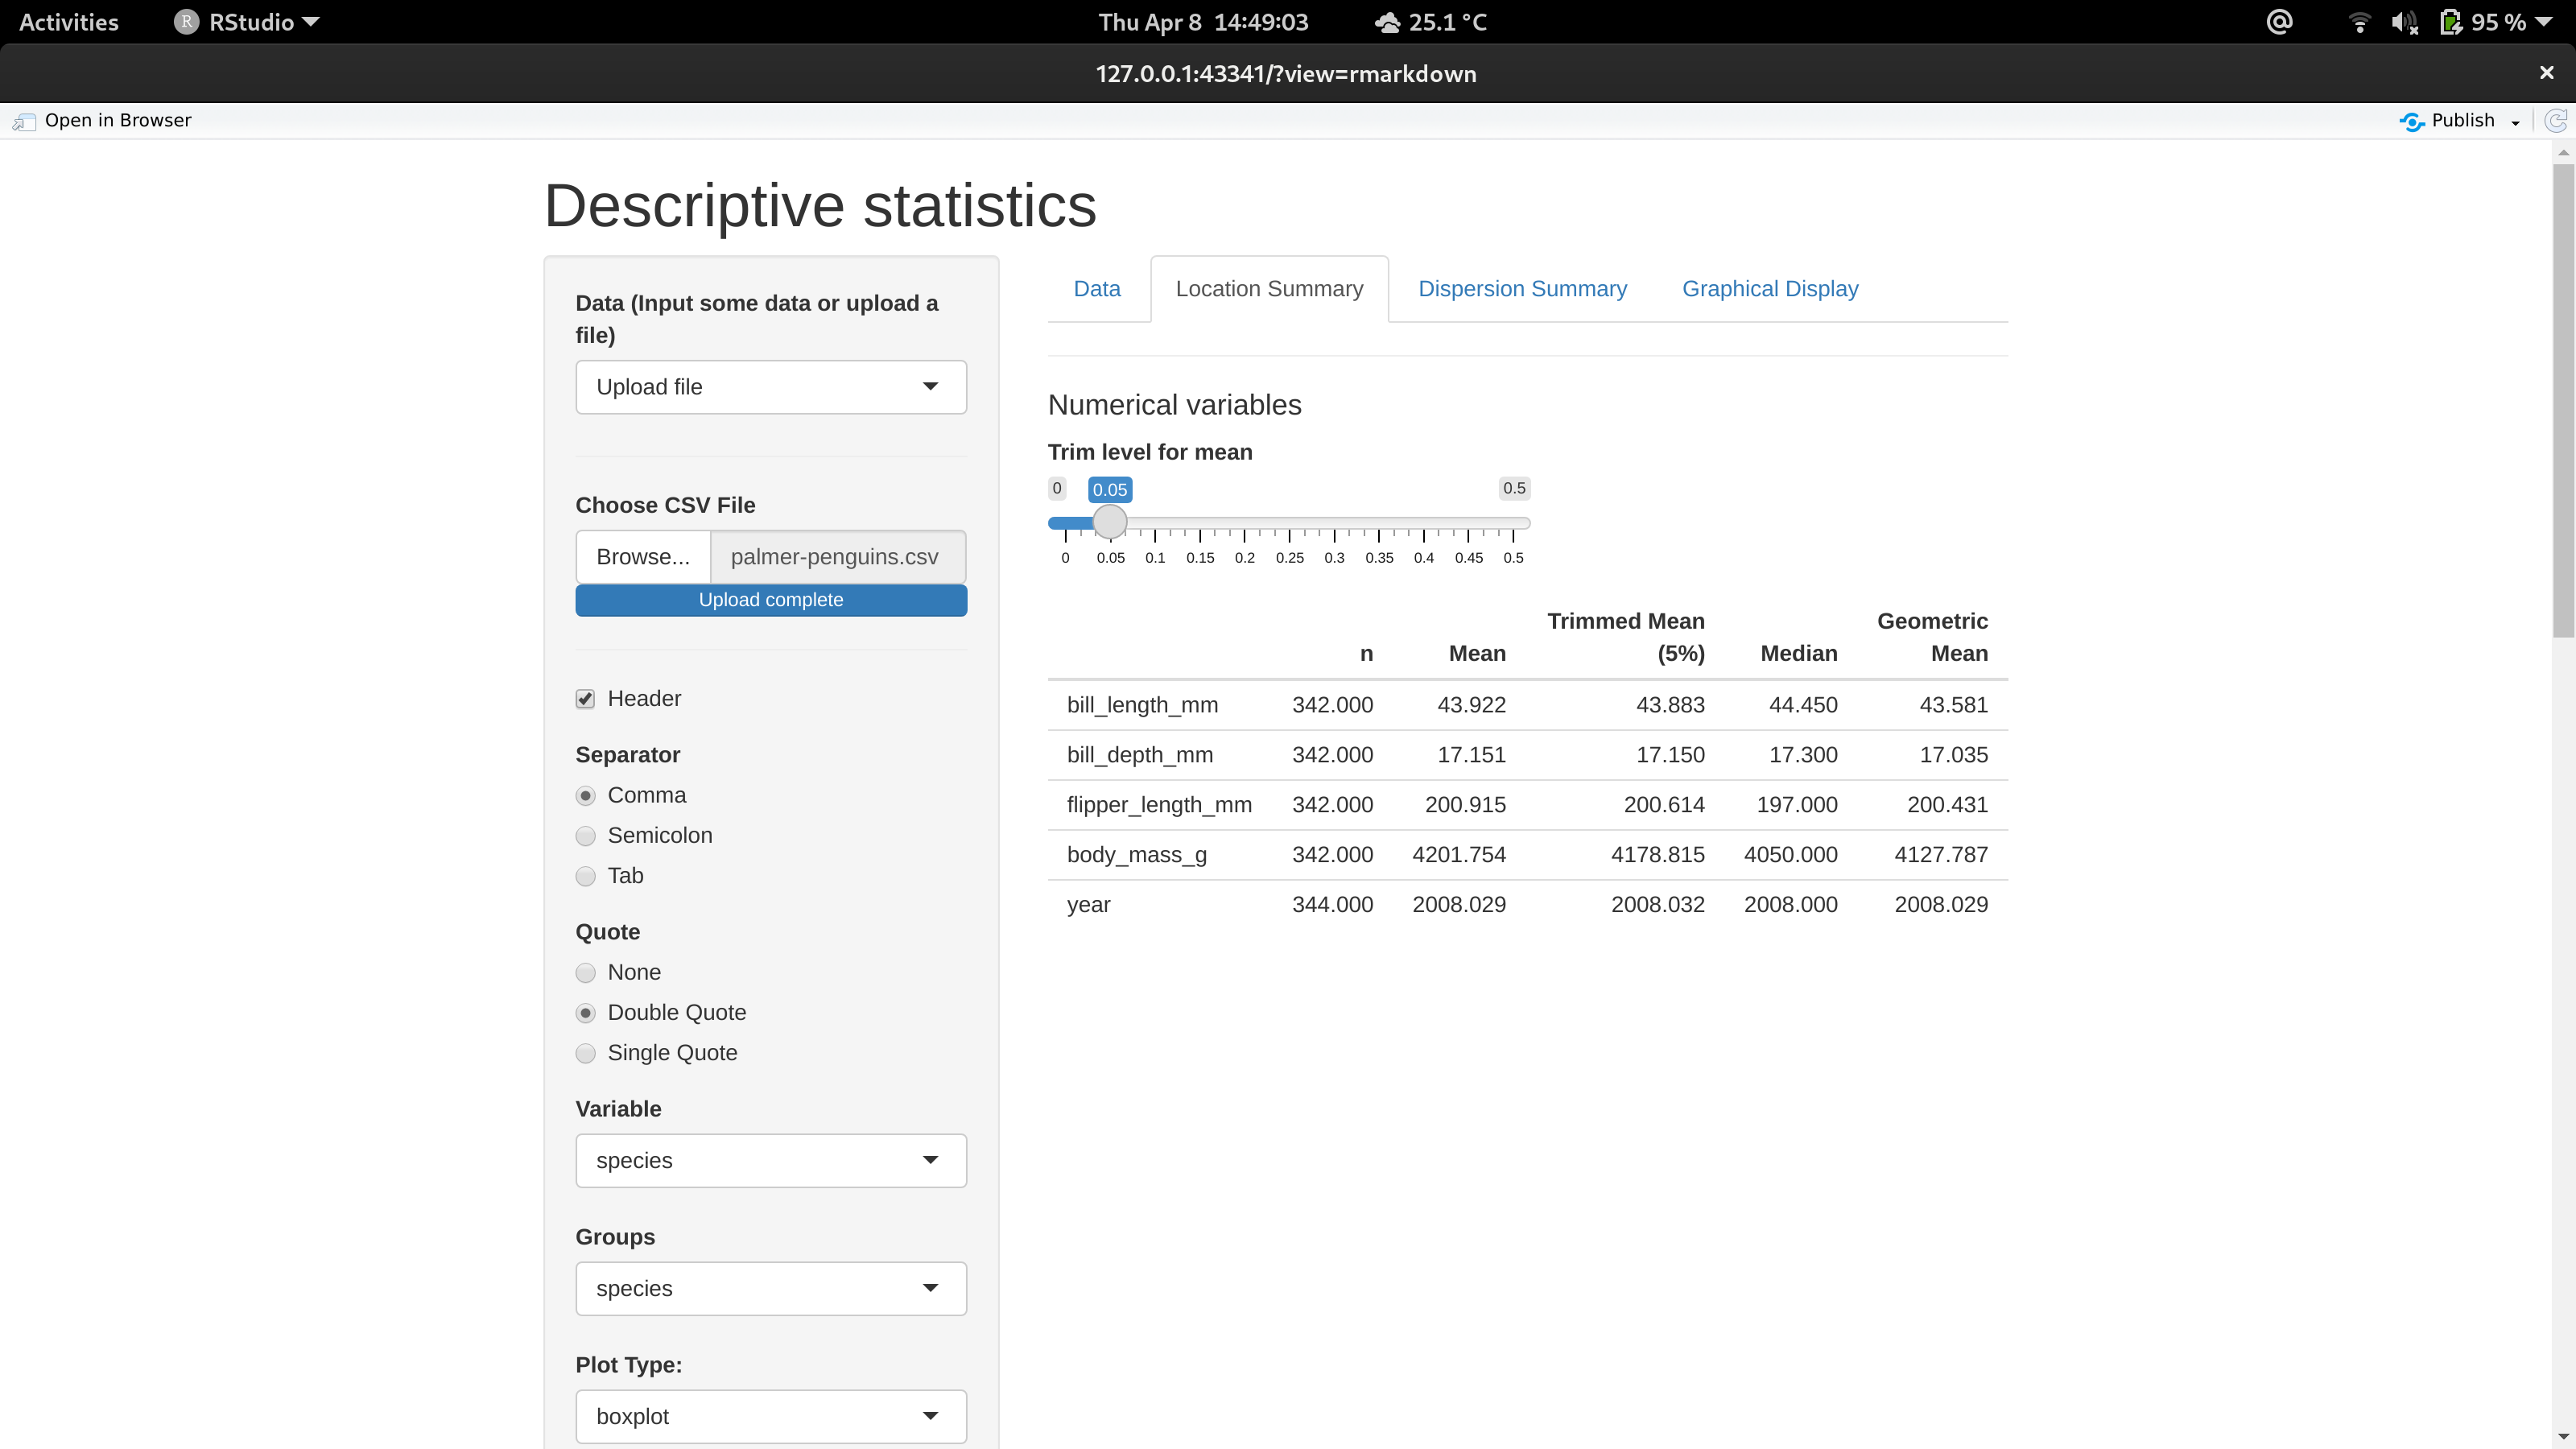
\includegraphics[width = \textwidth]{figures/Descriptive_2}
  \caption{Descriptive Statistics Web-page}\label{fig:DS2}
\end{figure}
